\documentclass[a4paper,12pt]{article}

\usepackage[english]{babel}
\usepackage{graphicx}
\graphicspath{{figures/}}

\setlength{\textheight}{25 cm}
\setlength{\textwidth}{16.5 cm}
\setlength{\oddsidemargin}{0.5 cm}
\setlength{\topmargin}{0 cm}
\setlength{\evensidemargin}{-0.5 cm}
\setlength{\footskip}{2\baselineskip}
\setlength{\headheight}{1\baselineskip}

\begin{document}

\hspace*{7cm} ISHEPP XV 28 September, 2000
\vspace*{5mm}

\begin{flushleft}
  {\Large\bf Deuteron as a Spin Flip Amplitude Analizer}

  {\large\bf (Charge Exchange Processes on the Deuteron)}
\end{flushleft}
\bigskip
    {\large\bf
      Yu.P. Bushuev$^{1}$,V.V. Glagolev$^{1}$, J. Hlav\'{a}\v{c}ov\'{a}$^{2}$,
      M.S. Khvastunov$^{1}$,\\D.A. Kirillov$^{1}$,
      N.B. Ladygina$^{1}$, G. Martinsk\'{a}$^{3}$, J. Mu\v sinsk\'y$^{1}$,\\
      B. Pastir\v c\'ak$^{4}$, N.M. Piskunov$^{1}$, A.A.Povtorejko$^{1}$, T. Siemiarczuk$^{5}$
      J.Urb\'{a}n$^{3}$ }\\

    \bigskip
    \hspace{-0.75cm}
    \small{$^{1}$Joint Institute for Nuclear Research,141980 Dubna,Russia\\
      $^{2}$Technical University, Park Komensk\'{e}ho 2, SK-04200, Ko\v{s}ice, Slovak Republic\\
      $^{3}$University of P.J.\v{S}af\'{a}rik, Jesenn\'{a} 5, SK-04154 Ko\v{s}ice, Slovak Republic \\
      $^{4}$Institute of Experimental Physics SAS, Watsonova 47, SK-04353, Ko\v{s}ice, Slovak Republic \\
      $^{5}$Institute of Nuclear Studies,ul. Hoza 69, Warsaw,  PL-00 681, Poland
      \\}

    \bigskip

    \begin{center}
      {\LARGE\bf Abstract}
    \end{center}
    \noindent
    \baselineskip=0.7cm
    \vspace*{1mm}

    {\large\bf An estimate of the spin dependent part of the np$\to$pn exchange
      amplitude has been made on the basis of the dp$\to$(pp)n data, taken
      by the 1m hydrogen bubble chamber in a full solid angle arrangement.
      At the momentum of 1.67 GeV/c per nucleon, as it has been shown, the
      np$\to$pn amplitude is entirely spin dependent. This result opens
      new possibilities for the experiments in polarized deuteron beams and
      polarized proton target.}

    {\large\bf An experiment is proposed to study the spin dependent part of the nucleon
      scattering amplitude in the   charge exchange process at the Nuclotron
      deuteron beams. The two-proton production cross section at small momentum
      transfers is intended to investigate in the range of
      the deuteron momentum from 3.0 GeV/c to 4.0 GeV/c. The experimental
      arrangement, the event selection methods and first test of STRELA setup
      on the NUCLOTRON are briefly reported.}

    \section{INTRODUCTION}
    \indent
    The task to build up the theory of the nucleon-nucleon scattering, specially
    for the region above 1 GeV, remains still actual. To have a complete sample
    of data what enables to carry out such informations as e.g. the phase analysis,
    experiments with double and triple scatterings are necessary. However, for investigation
    of the spin-flip contribution into the np$\to$pn charge exchange, the deuteron
    interacting with proton can be used, where the neutron is in a defined spin-orbital
    state.

    During the charge exchange process (the dp$\to$(pp)n reaction) of the deuteron
    breakup reaction, one of the two protons produced in a symmetrical spatial state has
    to change its spin state due to Pauli exclusive principle. So, the spin
    dependence of the elementary np$\to$pn charge exchange amplitude can be
    connected with the differential cross section at t=0. In this way the
    experiments in the deuteron beams can replace those with triple scatterings
    and enlarge the efficiency.

    Application of the above method to polarized deuteron beams can be used for
    proton tagging. Protons in aligned spin states allow to carry
    out experiments with  polarized proton targets on a much higher level.

    \section{EXPERIMENT}
    The experimental data have been taken by the JINR 1m hydrogen bubble
    chamber ~\cite{gla} in a full solid angle geometry, at a deuteron momentum of
    3.35 GeV/c. The use of nuclear
    beams impinging on a fixed proton target makes all the fragments of the
    incoming nuclei fast in the laboratory frame and, thus, they can be detected,
    well measured and identified practically without losses. On the other hand,
    almost all the losses due to the chamber threshold momenta are concentrated
    in the elastic channel. These conditions allow to study the reactions containing
    not more than one neutral particle in an exclusive approachs.

    The  dp$\to$ppn reaction can be divided
    into two channels:\\
    \begin{enumerate}
    \item the charge retention channel, where the proton is the fastest
      seconadary particle with respect to the deuteron rest frame and
    \item the charge exchange channel, where the neutron is the fastest
      secondary particle with respect to the deuteron rest frame.
    \end{enumerate}
    The separation of these two channels is illustrated in Fig. 1, showing
    the distribution of the four momentum transfer squared~t, between the impinging
    proton and the secondary neutron. Quantity defined in such a way does not
    depend on the final proton state, whether it is
    a spectator or it participates in the reaction
    (indifferent to the proton interferency).

    The first attempt to determine the contribution of the spin dependent
    amplitude of the np$\to$pn elementary charge exchange from the differential
    cross section of the dp$\to$(pp)n reaction \cite{Ala}, using the available
    pp and np scattering data, was carried out in the initial stage of the
    experiment on a relatively small part of the processed events. The data obtained
    as well as the estimate were ambigous because of the poor statistics.
    Nevertheless the enhanced role of the spin flip amplitude
    in the np$\to$pn charge exchange has been shown.

    We returned to this problem on the final statistics of over $10^{5}$ events of
    the dp$\to$ppn reaction for two reasons:
    \begin{enumerate}
    \item To estimate the dp$\to$(pp)n differential cross section
      at t=0 for the further use of the Dean formalism \cite{Dea}.
    \item To predict the capabilities and limitations of a prepared counter
      experiment \cite{Baz}.
    \end{enumerate}

    \section{RESULTS AND DISCUSSION}
    The possibility to use the charge exchange reaction on the unpolarized
    deuteron for determining the spin dependent part of the np$\to$pn charge
    exchange has been proposed by A.B. Migdal~\cite{Mig} and
    I.Y. Pomeranchuk~\cite{Pom}. The effect can be qualitatively understood in
    the following way. The nucleons bound in the deuteron may be in $^{3}S_{1}$
    and $^{3}D_{1}$ (T=0) spatial and spin symmetric states but their charge states
    should be antisymmetric. In the charge exchange process a charge
    symmetric state of two protons is produced and to fulfill the Pauli principle
    at a conserved spatial symmetry, the spin flip ( $^{1}S_{0}$ or $^{1}D_{2}$
    states of the two final protons )
    of the scattered nucleon ensures the asymmetric total wave function. In this
    way, the spin dependent part of the elementary charge exchange will be
    reflected through the probability of the charge exchange on the deuteron.

    The mathematical formalism within the impuls approximation was developed
    by Dean~\cite{Dea} and others. The general formula for the differential
    cross section of the dp$\to$(pp)n looks like:
    \begin{equation}
      \left( \frac{d\sigma }{dt}\right) (pd\rightarrow n(pp))=[1-F_d]\left(
      \frac{d\sigma _{nf}}{dt}\right) +[1-\frac{1}{3}F_d]
      \left(\frac{d\sigma _f}{dt}\right),
    \end{equation}
    where F$_d$ stands for the deuteron form factor, $\frac{d\sigma _{nf}}{dt}$ and
    $\frac{d\sigma _f}{dt}$ are non-spin flip and spin flip parts, respectively,
    of the np$\to$pn differential cross section. At zero transfers
    $(\vert t \vert\sim 0)$, when F$_d$=1 the expression (1) simplifies to:
    \begin{equation}
      \frac{d\sigma }{dt}(pd\rightarrow n(pp))=\frac 23\frac{d\sigma _f}
           {dt}(np\rightarrow pn).
    \end{equation}
    The last formula is applicable if at least two conditions are fulfilled:
    \begin{enumerate}
    \item the momentum transfer of the quasielastic np scattering is small,
    \item the intrinsic momenta q of the nucleons in the deuteron are small.
    \end{enumerate}

    The second condition means S-wave dominance in the deuteron wave function.
    It can be seen, e.g. in Fig 2, where the S wave probability distribution
    is shown as a function of the nucleons intrinsic momenta. In the region
    below p=0.07 GeV/c this probability practically does not depend on the nucleon
    intrinsic momenta.

    Both the above mentioned conditions can be fulfilled simultaneously, if one
    selects events in the laboratory frame ( fast deuteron impings on the proton
    target ) containing two fast protons  at small
    production angle, with momenta close
    to the half of the deuteron's one. We would like to emphasize, that this task
    can be realized successfully in the beams of accelerated deuterons.
    In the case of a deuteron target the two protons are too slow to be detected
    and the reaction cannot be identified.

    To answer the question of the spin flip contribution of the np$\to$pn process
    as it follows from expression (2), it is
    necesssary to turn to the experimental data on np$\to$pn charge exchange
    differential cross section at t=0. Such data have been obtained at Brookhaven
    \cite{Fri} for the region of 1-8 GeV and could be reasonably approximated
    by the function 1/p$^2$, where p is the momentum of the incoming
    neutron. The data imply ${d\sigma\over dt}$(0)=(36,9$\pm$ 3,0) $(GeV/c)^2$
    at 1.67 GeV/c.  The task now is to compare the differential cross section
    of the exchange on the deuteron, obtained in our experiment at t=0 with
    those for the np$\to$pn at the corresponding beam energy.

    For a reasonable approximation of $d\sigma/dt$ to t=0, it is inevitable
    to select a region of production angles, excluding the high momentum
    tails of the nucleon intrinsic motion and also the region of momentum
    transfers, where other more complicated mechanisms than the quasielastic
    scattering come into play. The differential cross sections
    for four different values of the two selected protons production angles are
    illustrated in Fig. 3.  The shape
    of the distribution at small $\vert t \vert$ does not change with the increase
    of the production angle while
    the contribution of higher $\vert t \vert$ increases.

    A typical value of the production angle is
    $\Theta=arctg(p_f/p_0)=1.6^{\circ}$, where
    the experimental and theoretical maxima ($p_f$=50 MeV/c) of the Fermi
    momentum distribution of the nucleons in the deuteron state as a measure
    of transverse momentum and the longitudinal momentum per nucleon
    in the laboratory frame is $p_0$=1.67 GeV/c.
    It leads to the result that the optimal value for the opening angle
    of a cone within the two
    protons are produced is around 3$^{\circ}$.

    In this connection we remind the used definitions: the slowest proton
    in the deuteron rest frame
    is referred to as a spectator; the other is the scattered one. If
    no cuts are imposed on the production angles of protons, their momentum
    distributions essentially differ as it is shown in Fig. 4. The spectator
    proton momentum distribution (full line) is of a shape, typical for the Fermi
    momentum distribution of the nucleon in the deuteron. When the above
    mentioned cut of 3$^\circ$ is applied to the spectator and scattered
    proton production angles, their momenta distributions, as one can see in Fig. 5,
    overlap. Their angular distributions are shown in Fig. 6.
    The quantity t is indifferent to the two proton
    interferency, as it has already been mentioned.

    The differential cross sections for small values of $\vert t\vert$ are
    displayed in Fig. 7 together with the curves, corresponding to a fit
    of ${d\sigma\over dt}$=ae $^{bt}$ to the data. The fit gives the
    following results: a=19,0$\pm$1,1
    ($\chi^2$/ND=4,3/8) for the interval of
    $\vert t\vert$=$\lbrace 0,0-0,02\rbrace$
    and  a=23,1${^+3,6 \atop _ -3,1}$
    ($\chi^2$/ND=1,0/2)
    for the interval
    $\vert t\vert$=$\lbrace 0,0-0,004 \rbrace$. Fig. 8 demonstrates
    the differential cross section at t=0 as a function of the cut, imposed
    on the proton production angles. It can be seen, that around $\theta$=3$^\circ$
    the quantity ${d\sigma\over dt}(0)$ reaches the level of
    ${2\over3}{d\sigma\over dt}(0)$ of the elementary np$\to$pn process.
    For the value of $\theta$=3$^\circ$ we get the contribution of the spin
    flip part to the elementary np$\to$pn of $0.94 \pm 0.15$. The obtained
    contribution of course depends on the unknown  systematical errors of the
    differential cross section of the elementary np$\to$pn charge exchange.
    In any case the contribution obtained is large enough and does not exclude
    the full spin flip in the np$\to$pn process. It means, that in the beams
    of vector  polarized deuterons one can get an additional possibility
    to use the studied reaction for more sophisticated purposes, e.g. to
    explain the interference mechanism in the two protons system. The
    spectator and the scattered protons are then tagged, because the first
    one conserves the beam polarization and the latter (scattered) is then
    polarized oppositely.

    \section{The new STRELA setup}
    The geometry, detectors and the background were estimated using:
    1) Monte Carlo simulations of the   reaction,
    2) real events from 17 different channels of dp interactions.
    The following parameters were used as inputs to the model: the spot of the
    deuteron beam at the target - 1 cm; the beam momentum - 3.5 GeV/c;
    the thickness of the liquid hydrogen target - 10 cm;
    the length of the magnet - 1m and the magnetic field fixing at 1 T;
    the distances from the target to the magnet 1m and to the first detector 7 m;
    the transverse size of the detector ~5 cm;
    the  Gartenhaus-Moravcsik deuteron wave function  and the experimental
    slopes of the Nd and NN elastic scattering.

    These parameters can be optimized according to the geometrical requirements
    of the setup. The experimental and Monte Carlo estimations of the background from the
    one-proton events of the   reaction, i.e. from the charge retention deuteron
    breakup, gave approximately the same results. It is expected not more
    than 400 one-proton events per one two-proton event, when the aperture
    of the event selection is ~0.5$^o$.
    The effect-background ratio improves by increasing this angle.

    In the case of one-proton events, the detected
    protons are spectators and they can give a good basis for the cross section
    normalization.

    Thus, two protons, each with half of the deuteron beam momentum, must be
    detected. This ensures that events at 0$^o$ with respect to the beam direction
    with small relative momentum of the nucleon internal motion in the deuteron
    and small transferred momentum to the scattered neutron are selected.
    Therefore the minimal necessary conditions for the detection of the proposed
    effect are possible to realize. On the first stage the experimental scheme,
    shown in Fig. 9, is proposed. The slow extraction deuteron beam is incident
    on a 10-cm liquid hydrogen target LH2 and the analyzing magnet D separates
    the primary deuterons and secondary particles. The ionization chamber IC
    measures a flux of the deuteron beam. The scintillator monitors T1-T3
    and M1-M2 control the intensity and position of the beam. The scintillator
    counters S1-S4 with diameters of 48 mm determine the angular and momentum
    acceptances (10$\%$) and trigger the event. The Cherenkov counters C1-C3 with
    polystirol radiators of the size 50*50*16 mm$^3$ select the two-proton events.
    The expected resolution about 10$\%$ allows to separate reliably the two
    and one-proton events. The Cherenkov counter C4 with a quartz radiator
    serves for pion suppression. The signal amplitudes from all counters are
    recorded for all the trigger events. To make the event selection more
    efficient, the possibility to include the signal amplitude from
    one of the Cherenkov counters in the trigger logic is foreseen.


    \section{Proposed data points, rates and first test of  STRELA setup}
    With 510$^{-2}$ msr angular acceptance and a momentum acceptance
    of 5$\%$ of the
    setup the proposed data points (2000 two proton events per energy) at
    the deuteron intensity of 10$^7$ per spill are given in the Table below.
    Each data point requires tuning of the Nuclotron and the additional time to
    check detectors and conditions of beam parameters, neither of them is included
    in to the time shown in the last coloumn of the table.
    \vspace*{5mm}

    \begin{tabular}{|c|c|c|c|c|c|}    \hline
      N    &    Td (GeV)&       Deuteron & One proton & Two proton & Time \\
      & &        momentum  & event  & events  & (min) \\
      & &(GeV/c)&       &       &       \\ \hline
      1   &     1.41 &  2.7  &  3100 &  8  &    50 \\  \hline
      2   &     1.49 &  2.8  &  3100 &  8  &    50 \\  \hline
      3   &     1.58 &  2.9  &  3100 &  8  &    50 \\  \hline
      4   &     1.66 &  3.0  &  3200 &  9  &    50 \\  \hline
      5   &     1.75 &  3.1  &  3200 &  9  &    50 \\  \hline
      6   &     1.83 &  3.2  &  3300 &  10 &    40 \\  \hline
      7   &     1.92 &  3.3 &   3400 &  10 &    40 \\  \hline
      8   &     2.00 &  3.4 &   3600 &  10 &    40 \\  \hline
      9   &     2.09 &  3.5 &   3800 &  11 &    40 \\  \hline
      10  &     2.18 &  3.6 &   4200 &  11 &    40 \\  \hline
      11  &     2.27 &  3.7 &   4400 &  12 &    40 \\  \hline
      12  &     2.36 &  3.8 &   4800 &  13 &    30 \\  \hline
      13  &     2.45 &  3.9 &   5100 &  14 &    30 \\  \hline
      14  &     2.54 &  4.0 &   5400 &  15 &    30 \\  \hline
    \end{tabular}
    \vspace*{5mm}

    In March,2000 the first run of STRELA setup on the extraction beam of NUCLOTRON
    has passed.
    The key possibility of adjustment of a telescope on a maximal stripping (Fig.10)
    and selections of two-proton events was shown (Fig.11).

    \section{CONCLUSION}
    \indent
    The study of the dp$\to$(pp)n reaction in full solid angle conditions
    has shown, that the amplitude of the elementary np$\to$pn charge exchange
    is fully spin dependent.
    The obtained result gives  new possibilities for experiments in polarized
    deuteron beams and polarized proton target.

    The first run of new experimental setup STRELA has been performed
    and the key possibility
    of obtaining new information about spin dependent amplitude np$\to$pn
    reaction in a wide range of energies has been shown.

    \begin{thebibliography}{99}
    \bibitem{gla} V.V.Glagolev, Nucl.Phys.B (Proc.Suppl.) 36 (1994) 509-512
    \bibitem{Ala} B.S.Aladashvili et al. //Nucl.Phys.B86, 1975, p.461
    \bibitem{Dea} N.W.Dean,//Phys.Rev.D5,1972,p.461

    \bibitem{Baz} S.N.Bazylev et al. Proc. Of the Int. Workshop
      "Relativistic nuclear physics from hundreds MeV to TeV", Slovak Republic,
      Stara Lesna, June 14-18, 1999, Dubna D1,2-99-294.

    \bibitem{Pom} I.Pomeranchuk DAN USSR, 1951, LXXVIII, N2, p.249
    \bibitem{Mig}   A.B.Migdal ZhETF 28, 1955, p.3
    \bibitem{Fri} J.L.Friedes et al.//Phys.Rev.Lett 15,1965,pp.38-41
    \bibitem{Ata} I.Atanasov et al. Research program of the Laboratory of
      High Energies, p.p.29-33, Dubna 99-266.

    \end{thebibliography}


    \section{FIGURE CAPTIONS}

    \noindent
    Fig.1. Distribution of four momentum transfer squared from the target proton
    to neutron for the dp$\to$ppn events. \\

    \noindent
    Fig.2. The S wave probability as a function of the nucleon Fermi momentum. \\

    \noindent
    Fig.3. Distribution of $\vert t \vert$ for the charge exchange channel with
    the
    production angles of both protons below 2,3,4 and 5 degrees. \\

    \noindent
    Fig. 4. Momentum distributions of the spectator ( full line)
    and  the scattered proton (dashed line) in the deuteron rest frame. \\

    \noindent
    Fig. 5. Momentum distributions of the spectator ( full line) and
    the scattered proton (dashed line) in the deuteron rest frame. The proton production angles
    in the laboratory frame are below 3$^{\circ}$. \\

    \noindent
    Fig. 6. Angular distribution of the spectator proton (full line) and that
    of the scattered one (dashed line) in the deuteron rest frame, for the case when their
    production angle in the laboratory frame is in the interval 0-3$^{\circ}$. \\

    \noindent
    Fig. 7. Differential cross section of the charge exchange reaction in
    the region of small $\vert t \vert$. The production angle of both protons
    in the laboratory frame is in the interval 0-3$^{\circ}$. \\

    \noindent
    Fig. 8. Differential cross section at t=0 when both protons are within
    a cone of opening angle $\Theta$. \\

    \noindent
    Fig.9.  Layout of the experimental setup. \\

    \noindent
    Fig.10. Experimental and Monte Carlo distributions of stripping protons.\\

    \noindent
    Fig.11. Cherenkov amplitude for one- and two-proton events.\\

    % ******* Figure 1 *********
    \begin{figure}[hbt]
      \begin{center}
        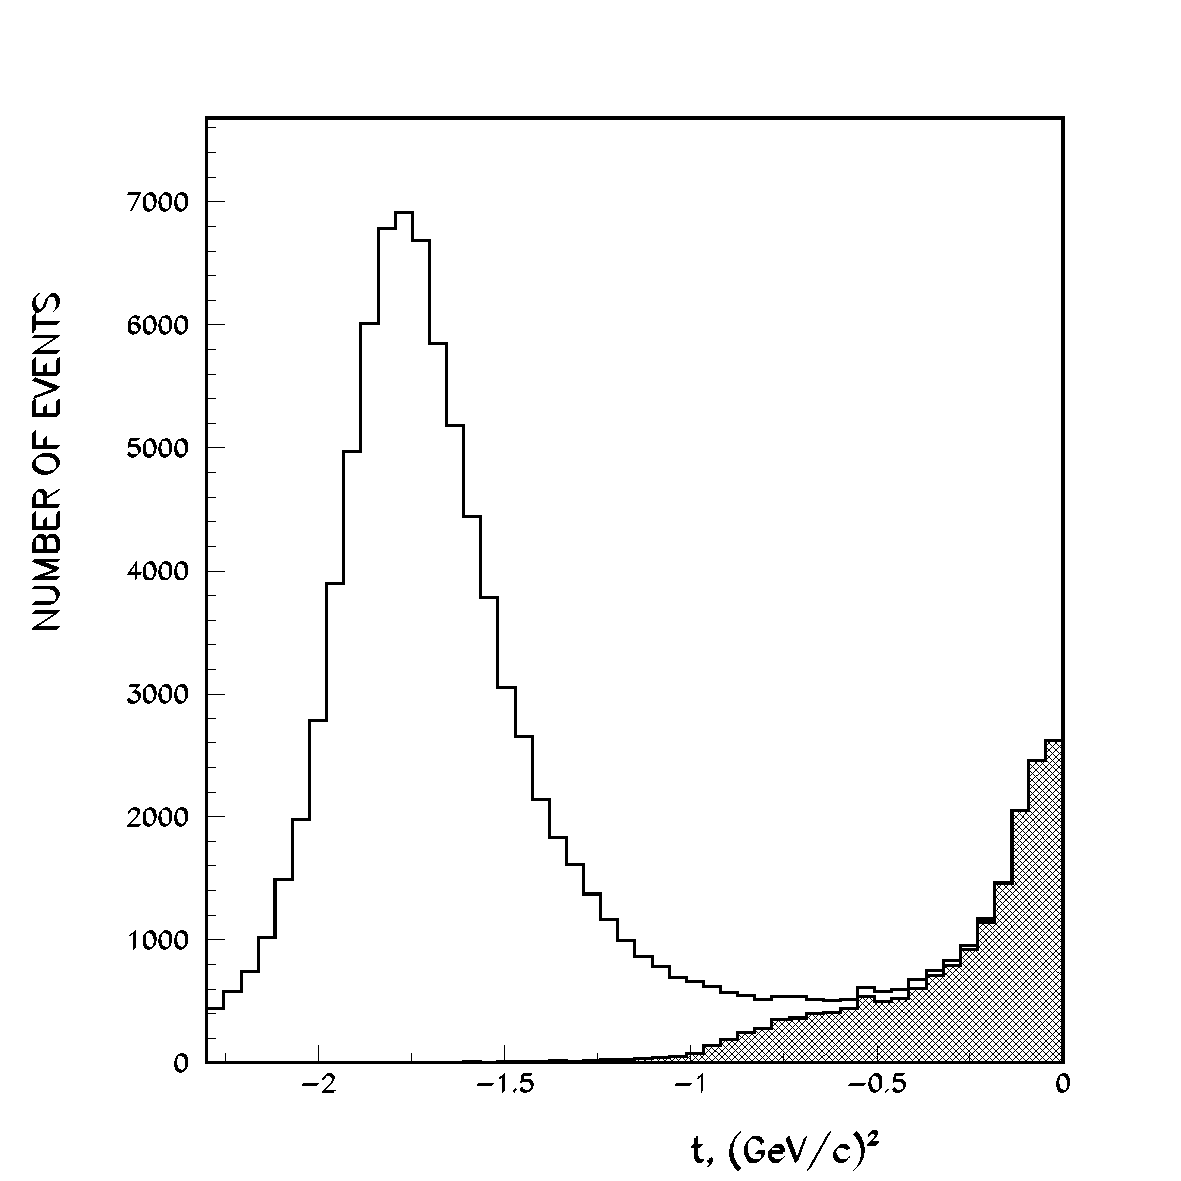
\includegraphics[width=8cm]{dist.pdf}
        %\mbox{\epsfig{figure=dist.eps,width=8.cm}}
      \end{center}
      \vspace{0.4mm}
      Fig.1.

    \end{figure}

    % ******* Figure 2 *********
    \begin{figure}[hbt]
      \begin{center}
        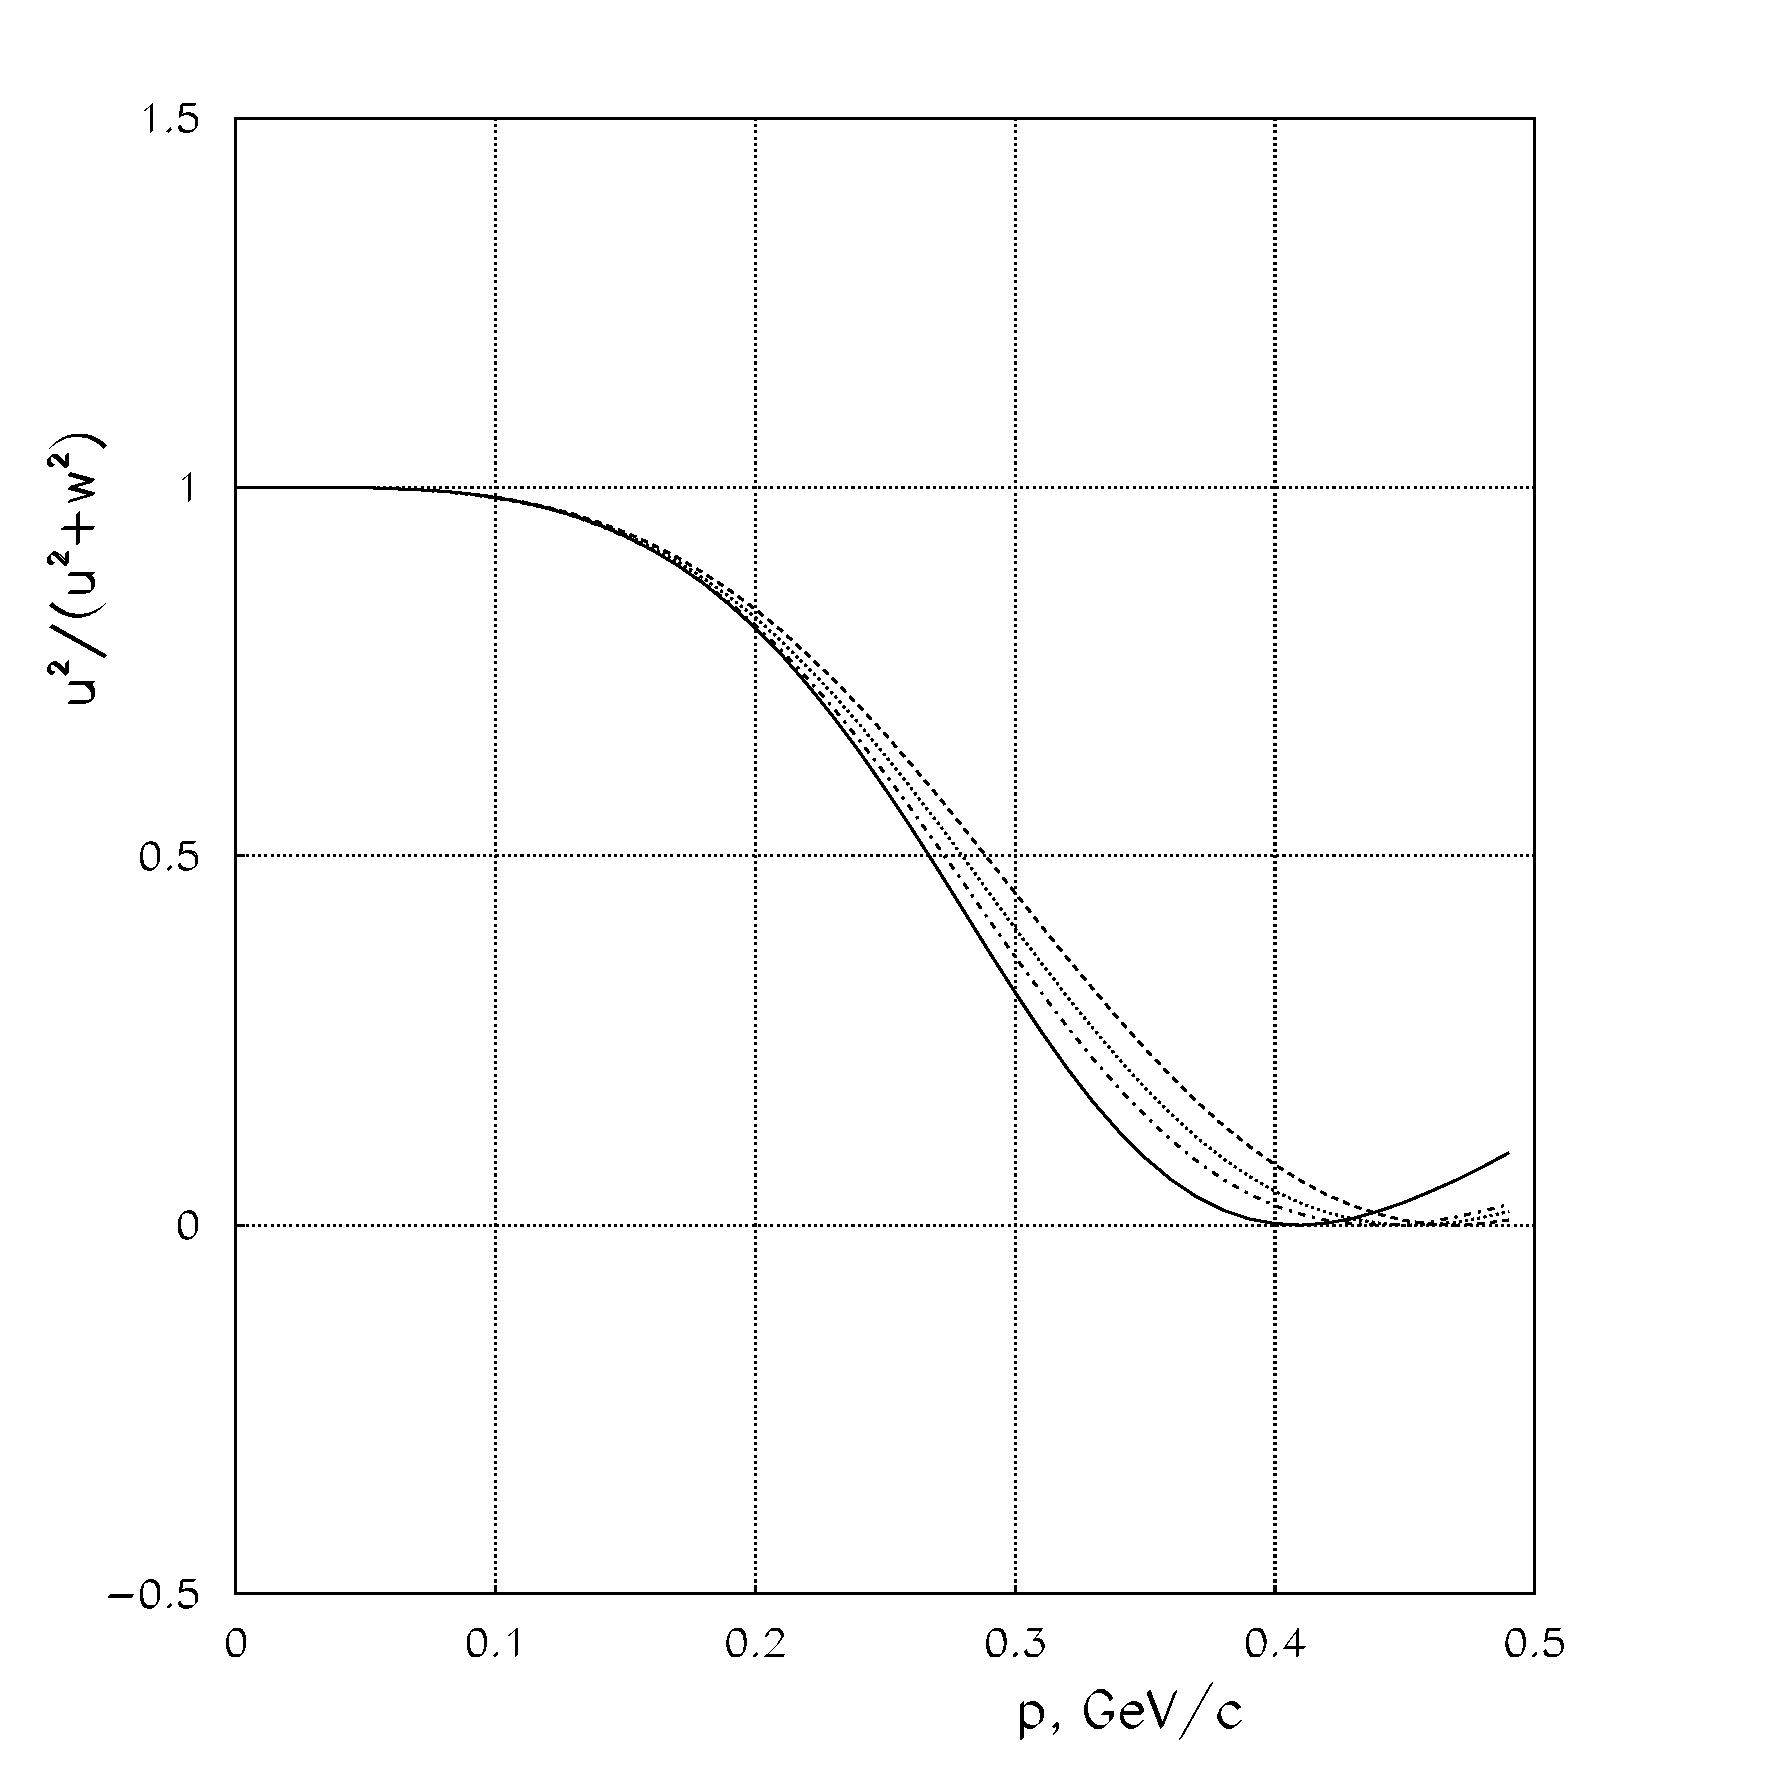
\includegraphics[width=8cm]{wavedtr.pdf}
        %\mbox{\epsfig{figure=wavedtr.eps,width=8.cm}}
      \end{center}
      \vspace{0.4mm}
      Fig.2.
    \end{figure}
    \newpage
    \newpage
    % ******* Figure 3 *********
    \begin{figure}[hbt]
      \begin{center}
        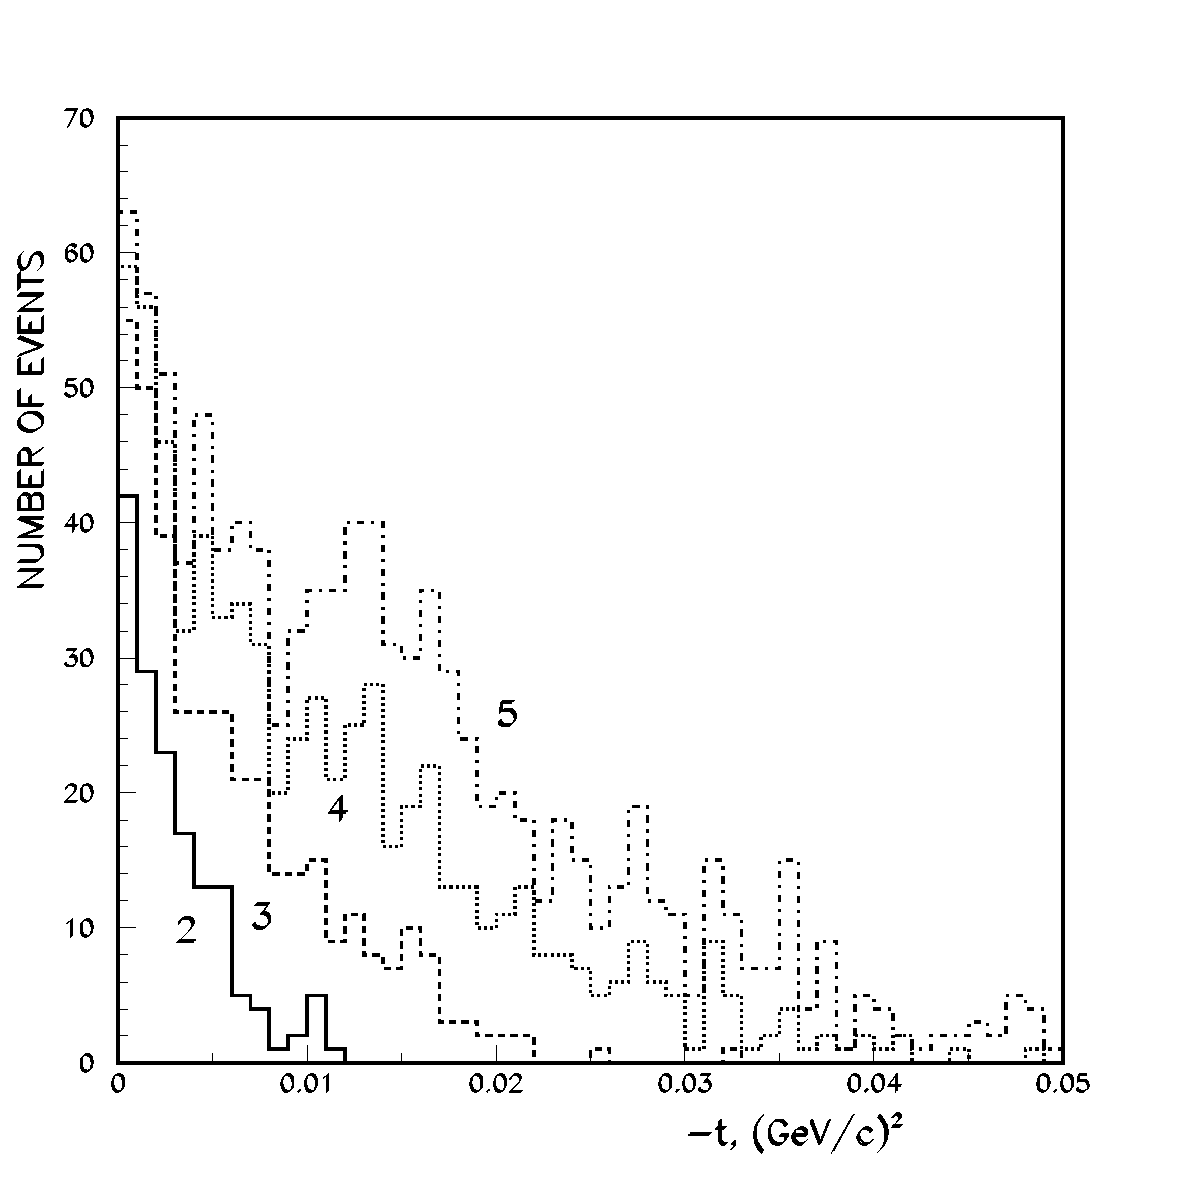
\includegraphics[width=8cm]{tpp2345.pdf}
        %\mbox{\epsfig{figure=tpp2345.eps,width=8.cm}}
      \end{center}
      \vspace {0,4cm}
      Fig.3.
    \end {figure}
    % ******* Figure 4 *********
    \begin{figure}[hbt]
      \begin{center}
        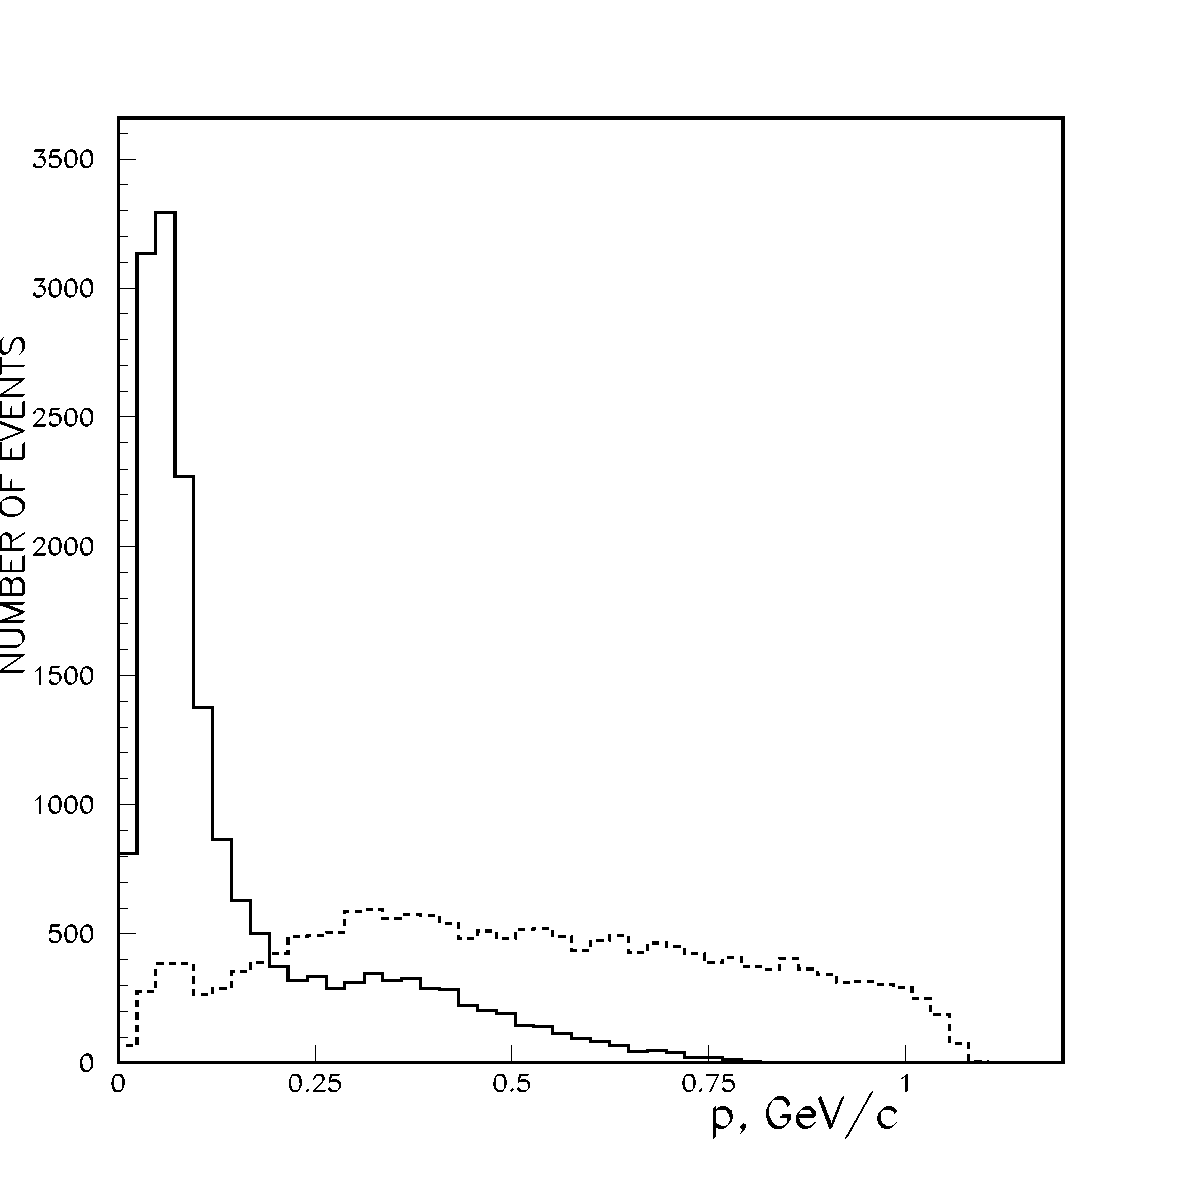
\includegraphics[width=8cm]{mompp.pdf}
        %\mbox{\epsfig{figure=mompp.eps,width=8.cm}}
      \end{center}
      \vspace {0.4cm}
      Fig.4.
    \end{figure}
    \newpage
    % ******* Figure 5 *********
    \begin{figure}[hbt]
      \begin{center}
        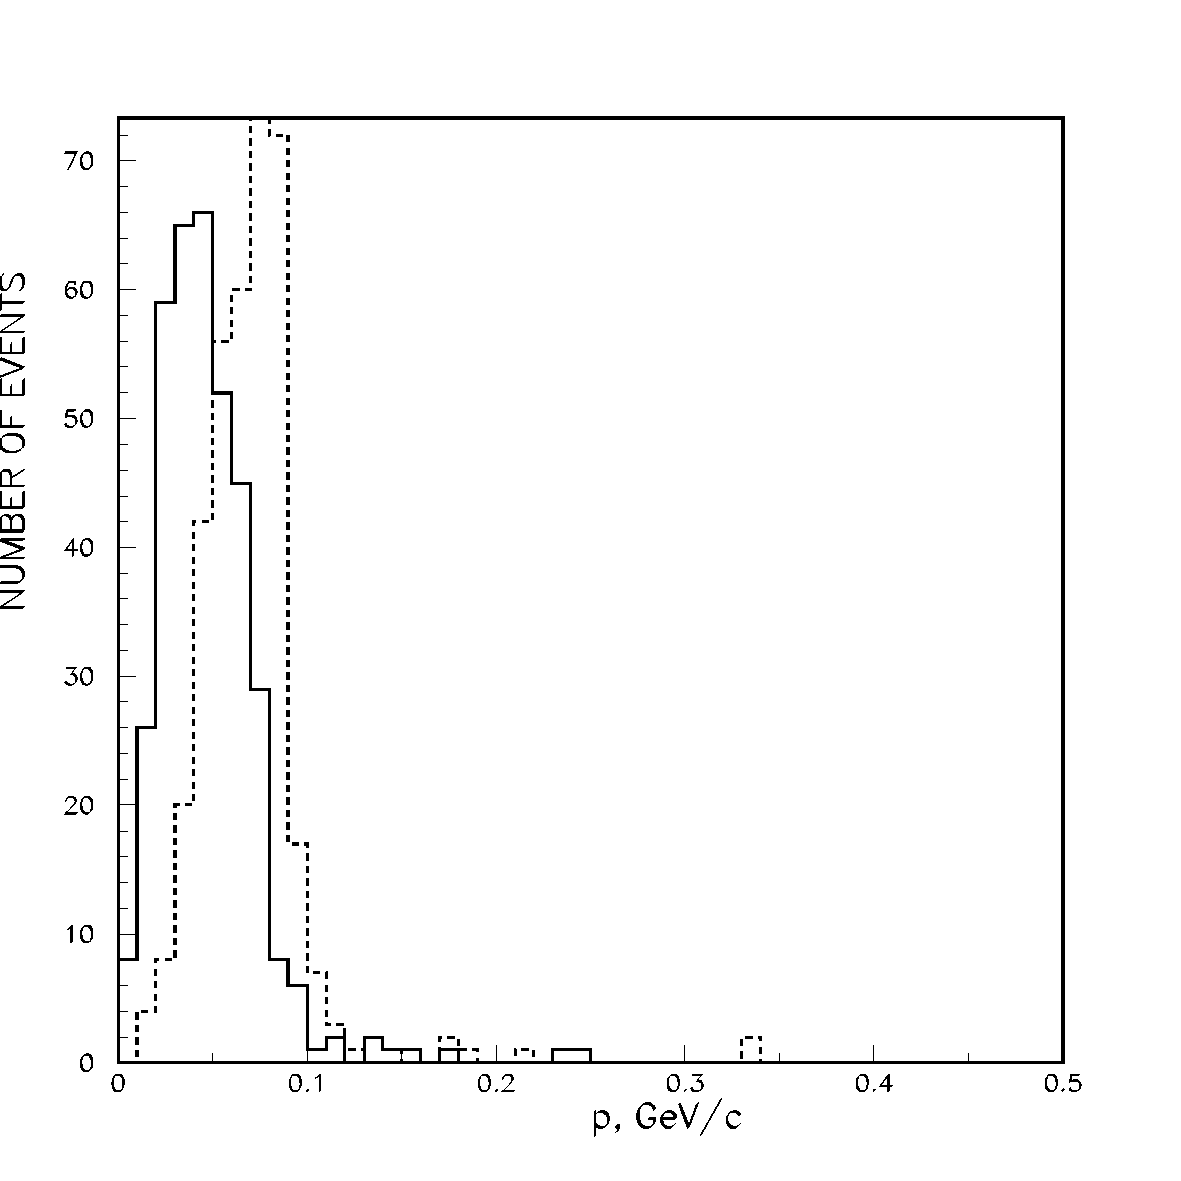
\includegraphics[width=8cm]{mom3d.pdf}
        %\mbox{\epsfig{figure=mom3d.eps,width=8.cm}}
      \end{center}
      \vspace {0.4cm}
      Fig.5.
    \end{figure}

    % ******* Figure 6 *********
    \begin{figure}[h]
      \begin{center}
        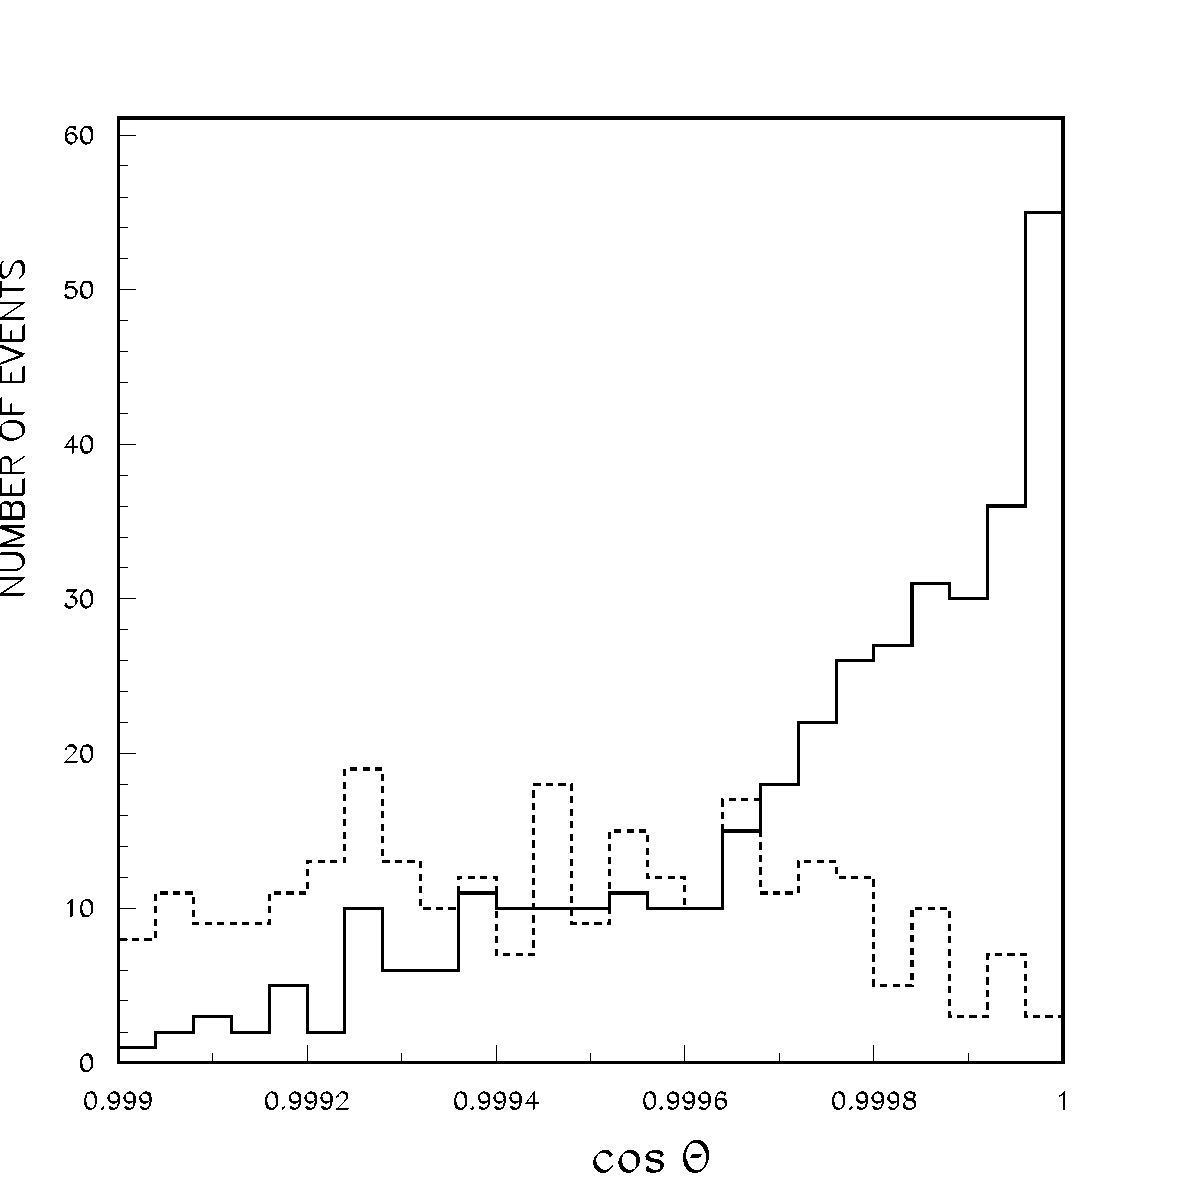
\includegraphics[width=8cm]{cospp.pdf}
        %\mbox{\epsfig{figure=cospp.eps,width=8.cm}}
      \end{center}
      \vspace{0,4mm}
      Fig.6
    \end{figure}
    \newpage
    \newpage
    % ******* Figure 7 *********
    \begin{figure}[hbt]
      \begin{center}
        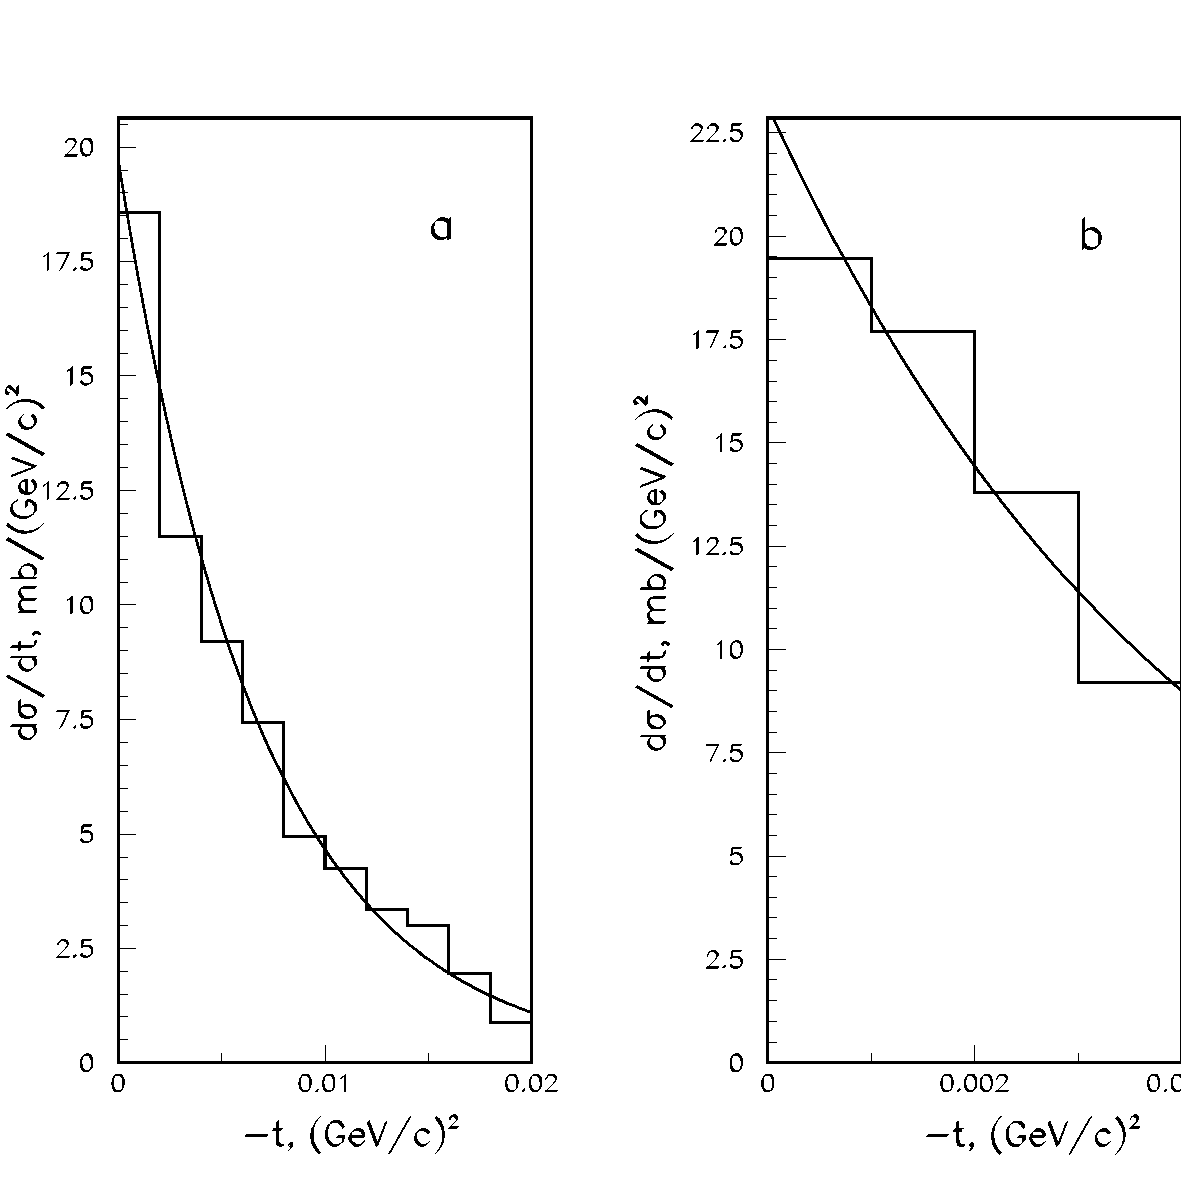
\includegraphics[width=8cm]{ppnce.pdf}
        %\mbox{\epsfig{figure=ppnce.eps,width=8.cm}}
      \end{center}
      \vspace{0,4mm}
      Fig.7.
    \end{figure}
    % ******* Figure 8 *********
    \begin{figure}[hbt]
      \begin{center}
        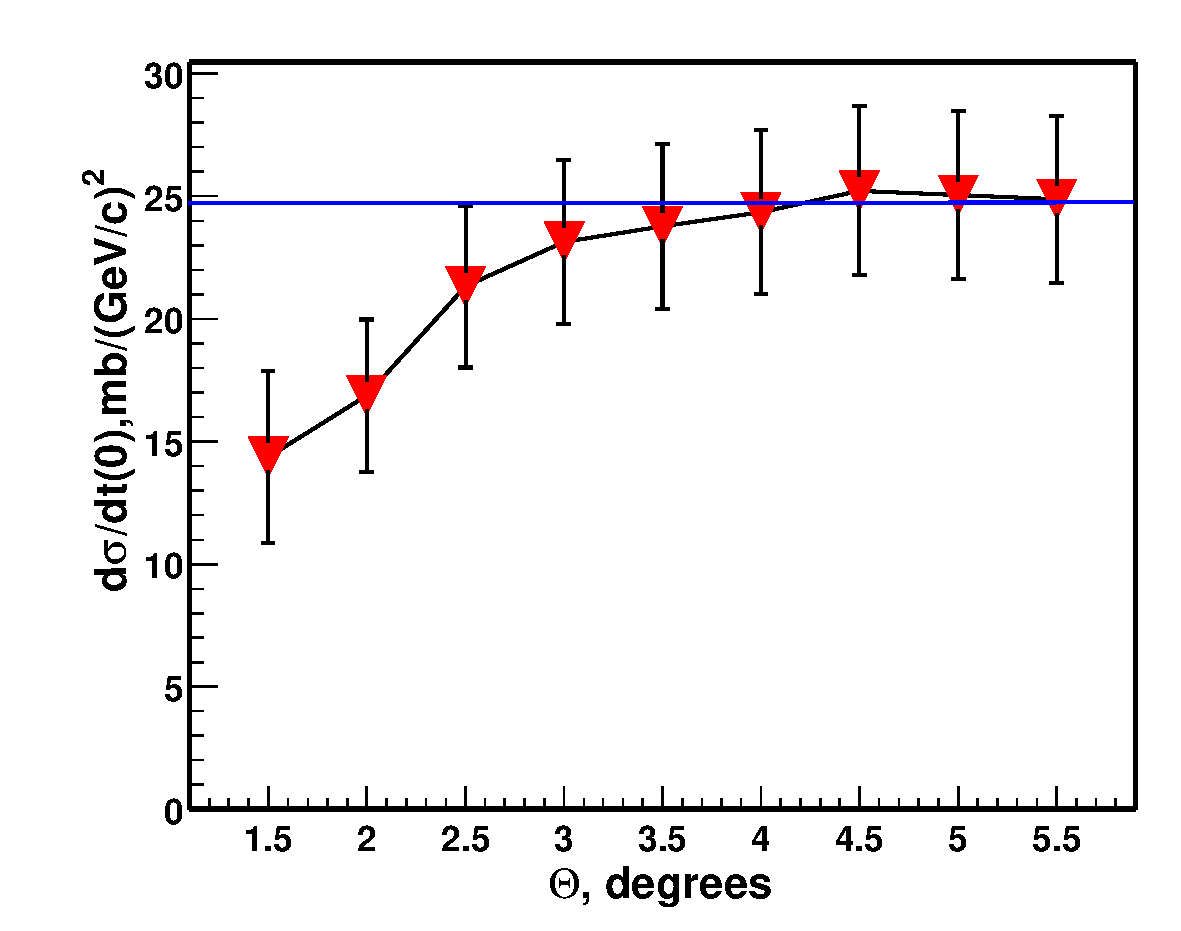
\includegraphics[width=8cm]{sigma0.pdf}
        %\mbox{\epsfig{figure=sigma0.eps,width=8.cm}}
      \end{center}
      \vspace{0,4mm}
      Fig.8.
    \end{figure}

    % ******* Figure 9 *********
    \begin{figure}[hbt]
      \begin{center}
        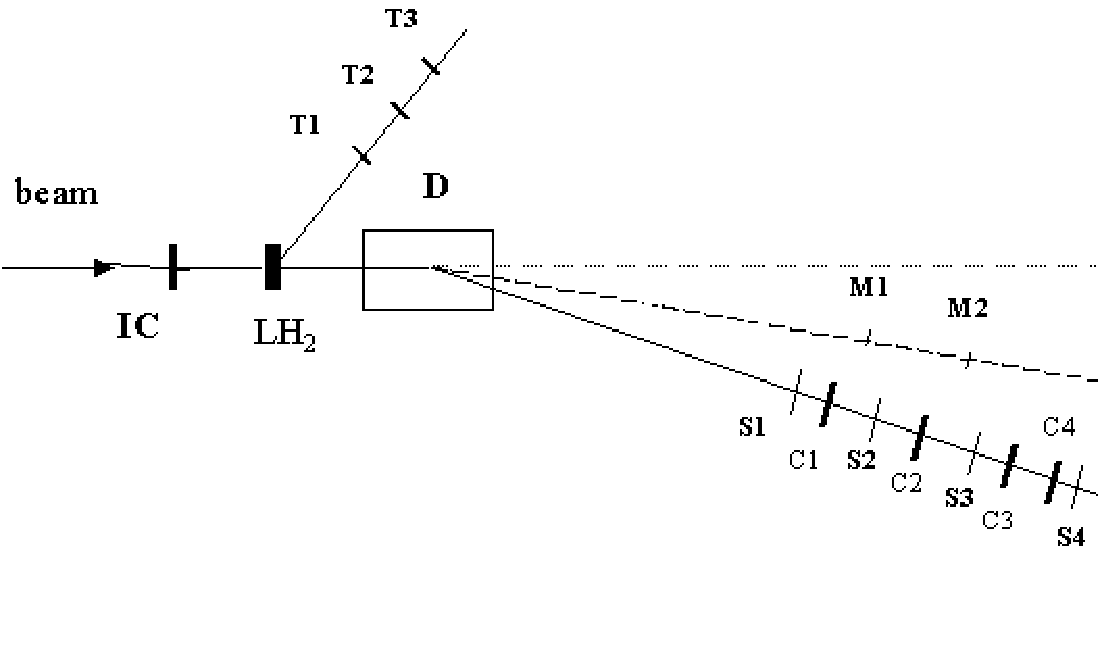
\includegraphics[width=8cm]{image2.pdf}
        %\mbox{\epsfig{figure=Image2.eps,width=8.cm}}
      \end{center}
      \vspace{0,4mm}
      Fig.9.
    \end{figure}


    % ******* Figure 10 *********
    \begin{figure}[hbt]
      \begin{center}
        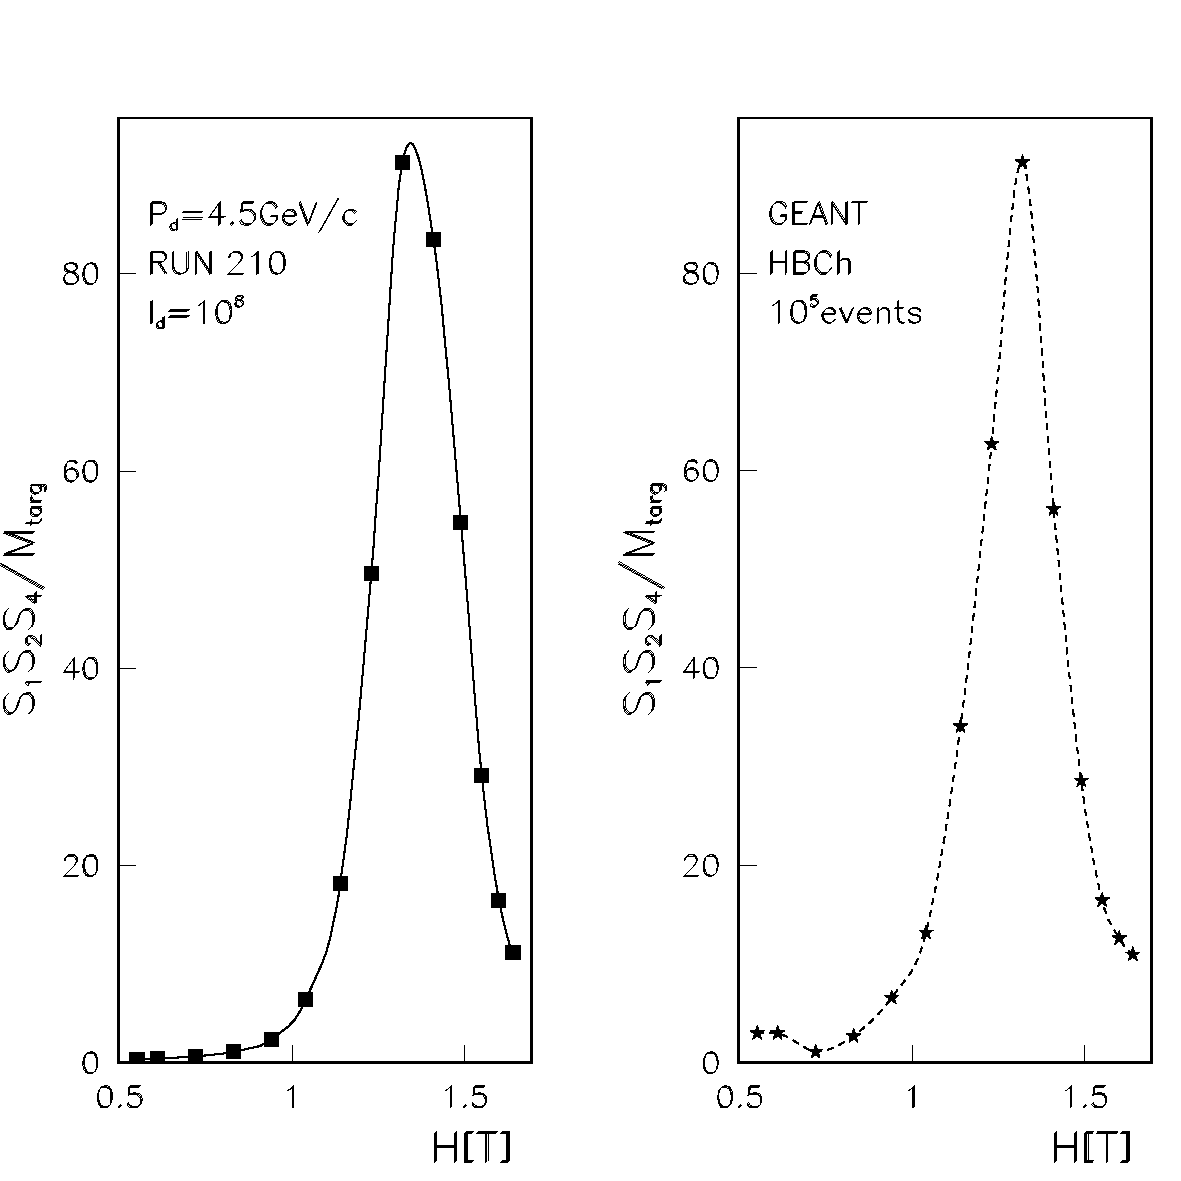
\includegraphics[width=8cm]{s3ok.pdf}
        %\mbox{\epsfig{figure=S3ok.eps,width=8.cm}}
      \end{center}
      \vspace{0,4mm}
      Fig.10.
    \end{figure}


    % ******* Figure 11 *********
    \begin{figure}[hbt]
      \begin{center}
        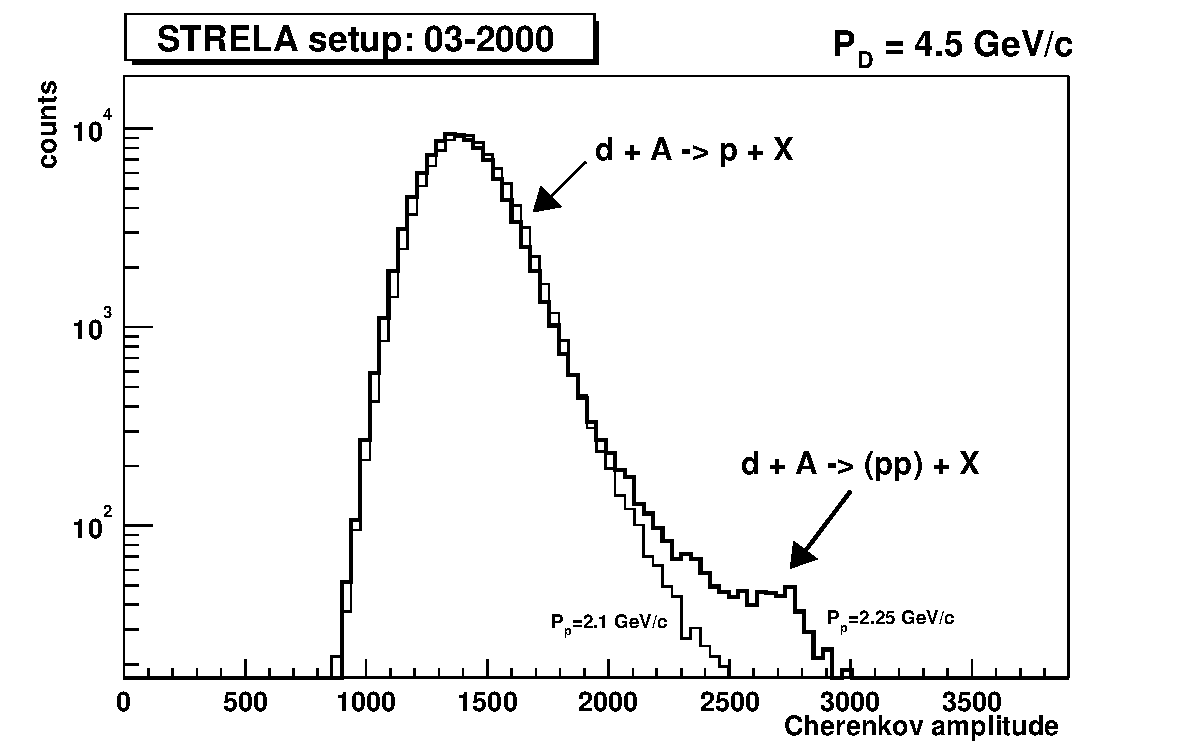
\includegraphics[width=8cm]{strela.pdf}
        %\mbox{\epsfig{figure=strela.eps,width=8.cm,angle=0}}
      \end{center}
      \vspace{0,4mm}
      Fig.11.
    \end{figure}

\end{document}
